\documentclass{article}
\usepackage[utf8]{inputenc}
\usepackage[margin=2.6cm]{geometry}
\usepackage{float}
\usepackage{rotating}
\usepackage{graphicx}
\usepackage{caption}
\usepackage{subcaption}
\usepackage[round]{natbib}
\usepackage{setspace}
\usepackage{longtable}
\usepackage{lscape}
\onehalfspacing
\usepackage{tikz}
\usetikzlibrary{arrows,automata,positioning,shapes}


\begin{document}

\begin{figure}
\centering
\begin{minipage}{.47\textwidth}
\centering
\vfill
  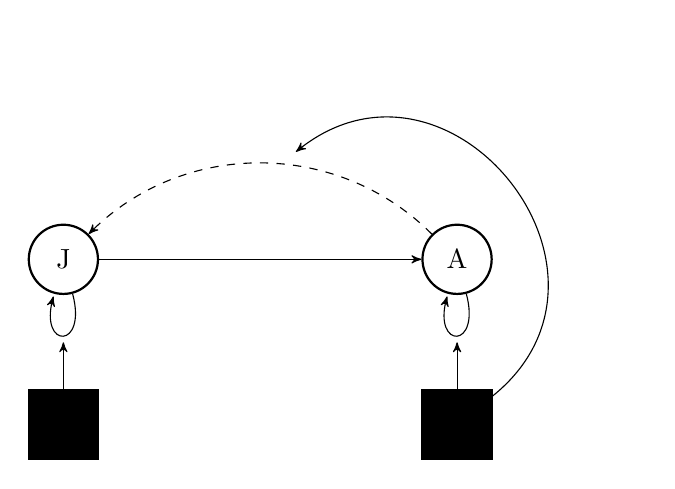
\begin{tikzpicture}[->,>=stealth',auto,thin]
\tikzstyle{every state}=[fill=white,shape=rectangle,draw,thick,text=black, text centered, text width=0.5cm, align=center]

\node[state]        (A) [shape=circle]        {J};
\node[state]		(B) [below of=A,node distance=0.6cm,draw=none,fill=none] {};
\node[state]		(C) [below of=B,node distance=1.5cm,fill=black] {};
\node[state]        (D) [right of=A,shape=circle, node distance=5cm] {A};
\node[state]		(E) [below of=D,node distance=0.6cm,draw=none,fill=none] {};
\node[state]		(F) [below of=E,node distance=1.5cm,fill=black] {};
\node[state]        (G) [right of=A,node distance=2.5cm,draw=none,fill=none] {};
\node[state]        (H) [above of=G,node distance=1cm,draw=none,fill=none] {};

\path
(A) edge[loop below] (A)
(C) edge (B)
(A) edge (D)
(D) edge[loop below] (D)
(D) edge[dashed,bend left=-45] (A)
(F) edge (E)
(F) edge[bend right=90, min distance=2.5cm] (H)
;
    \end{tikzpicture}
 \vfill
\captionsetup{labelformat=empty}
\caption{1) Black box resource dynamics model}
\label{fig:blackbox}
\vspace{\baselineskip}
\end{minipage}\qquad
\begin{minipage}{.47\textwidth}
\centering
\vfill
\begin{tikzpicture}[->,>=stealth',auto,thin,]
\tikzstyle{every state}=[fill=white,shape=rectangle,draw,thick,text=black, text centered, text width=0.5cm, align=center]

\node[state]        (A) [shape=circle]        {J};
\node[state]		(B) [below of=A,node distance=0.6cm,draw=none,fill=none] {};
\node[state]		(C) [below left of=B,node distance=1.5cm] {R$_J$};
\node[state]        (D) [below right of=B,node distance=1.5cm] {S$_J$};
\node[state]        (E) [right of=A, node distance=5cm,shape=circle] {A};
\node[state]		(F) [below of=E,node distance=0.6cm,draw=none,fill=none] {};
\node[state]		(G) [below left of=F,node distance=1.5cm] {G$_A$};
\node[state]		(I) [below of=F,node distance=2.5cm] {P$_A$};
\node[state]        (J) [below right of=F,node distance=1.5cm] {S$_A$};
\node[state]        (K) [right of=A,node distance=2.5cm,draw=none,fill=none] {};
\node[state]        (L) [above of=K,node distance=1cm,draw=none,fill=none] {};

\path
(A) edge[loop below] (A)
(C) edge (D)
(D) edge (B)
(C) edge (D)
(A) edge (E)
(E) edge[loop below] (E)
(E) edge[dashed,bend left=-45] (A)
(I) edge (G)
(I) edge (J)
(I) edge[bend right=100, min distance=4cm] (L)
(J) edge (F)
;
    \end{tikzpicture}
\vfill
\captionsetup{labelformat=empty}
\caption{2) Embodied capital model}
\label{fig:embodied}
\end{minipage}

\begin{minipage}{.41\textwidth}
\centering
\vfill
      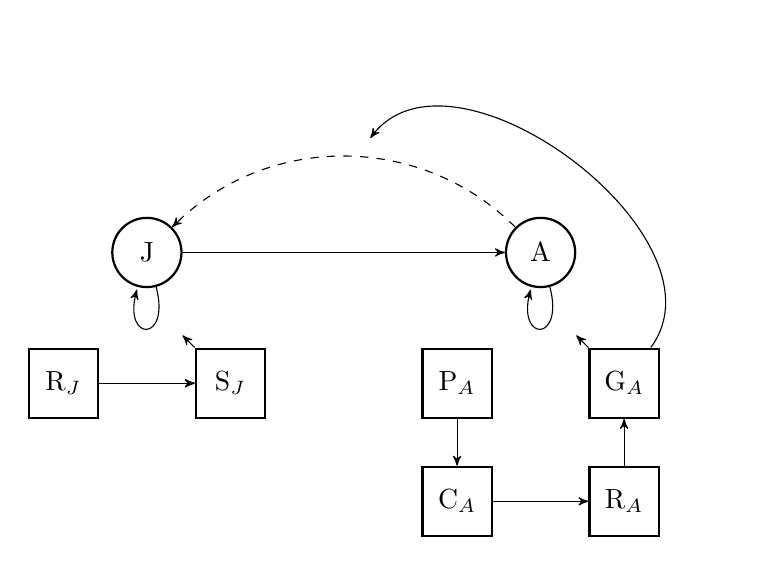
\begin{tikzpicture}[->,>=stealth',auto,thin]
\tikzstyle{every state}=[fill=white,shape=rectangle,draw,thick,text=black, text centered, text width=0.5cm, align=center]

\node[state]        (A) [shape=circle]        {J};
\node[state]		(B) [below of=A,node distance=0.6cm,draw=none,fill=none] {};
\node[state]		(C) [below left of=B,node distance=1.5cm] {R$_J$};
\node[state]        (D) [below right of=B,node distance=1.5cm] {S$_J$};
\node[state]        (E) [right of=A, node distance=5cm,shape=circle] {A};
\node[state]		(F) [below of=E,node distance=0.6cm,draw=none,fill=none] {};
\node[state]		(G) [below left of=F,node distance=1.5cm] {P$_A$};
\node[state]		(I) [below of=G,node distance=1.5cm] {C$_A$};
\node[state]        (J) [below right of=F,node distance=1.5cm] {G$_A$};
\node[state]        (K) [below of=J,node distance=1.5cm,] {R$_A$};
\node[state]        (L) [right of=A,node distance=2.5cm,draw=none,fill=none] {};
\node[state]        (M) [above of=L,node distance=1cm,draw=none,fill=none] {};

\path
(A) edge[loop below] (A)
(C) edge (D)
(D) edge (B)
(C) edge (D)
(A) edge (E)
(E) edge[loop below] (E)
(E) edge[dashed,bend left=-45] (A)
(G) edge (I)
(I) edge (K)
(J) edge[bend right=90, min distance=1.5cm] (M)
(J) edge (F)
(K) edge (J)
;
    \end{tikzpicture}
 \vfill
\captionsetup{labelformat=empty}
\caption{3) Inter-generational resource transfer model}
\label{fig:transfer}
\end{minipage}\qquad
\begin{minipage}{.5\textwidth}
\centering
\vfill
    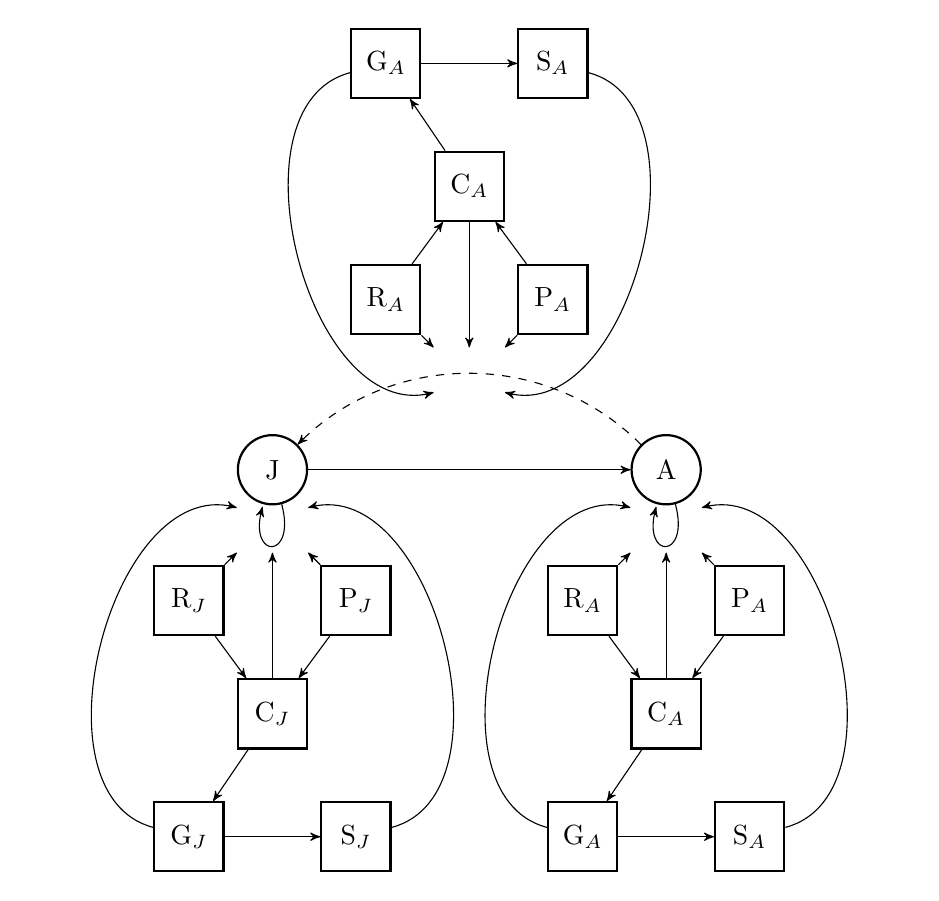
\begin{tikzpicture}[->,>=stealth',auto,thin]
\tikzstyle{every state}=[fill=white,shape=rectangle,draw,thick,text=black, text centered, text width=0.5cm, align=center]

\node[state]        (A) [shape=circle]        {J};
\node[state]		(B) [below of=A,node distance=0.6cm,draw=none,fill=none] {};
\node[state]		(C) [below left of=B,node distance=1.5cm] {R$_J$};
\node[state]        (D) [below of=C,node distance=3cm] {G$_J$};
\node[state]		(E) [below of=B,node distance=2.5cm] {C$_J$};
\node[state]        (F) [below right of=B,node distance=1.5cm] {P$_J$};
\node[state]		(G) [below of=F,node distance=3cm] {S$_J$};
\node[state]        (H) [right of=A, node distance=5cm,shape=circle] {A};
\node[state]		(I) [below of=H,node distance=0.6cm,draw=none,fill=none] {};
\node[state]		(J) [below left of=I,node distance=1.5cm] {R$_A$};
\node[state]		(K) [below of=J,node distance=3cm] {G$_A$};
\node[state]		(L) [below of=I,node distance=2.5cm] {C$_A$};
\node[state]        (M) [below right of=I,node distance=1.5cm] {P$_A$};
\node[state]		(N) [below of=M,node distance=3cm] {S$_A$};
\node[state]        (O) [right of=A,node distance=2.5cm,draw=none,fill=none] {};
\node[state]        (P) [above of=O,node distance=1.1cm,draw=none,fill=none] {};
\node[state]		(Q) [above left of=P,node distance=1.5cm] {R$_A$};
\node[state]		(R) [above of=Q,node distance=3cm] {G$_A$};
\node[state]		(S) [above of=P,node distance=2.5cm] {C$_A$};
\node[state]        (T) [above right of=P,node distance=1.5cm] {P$_A$};
\node[state]		(U) [above of=T,node distance=3cm] {S$_A$};

\path
(A) edge[loop below] (A)
(C) edge (B)
(C) edge (E)
(D) edge[bend right=-90] (B)
(D) edge (G)
(E) edge (B)
(E) edge (D)
(F) edge (B)
(F) edge (E)
(G) edge[bend left=-90] (B)
(A) edge (H)
(H) edge[loop below] (H)
(H) edge[dashed,bend left=-45] (A)
(J) edge (I)
(J) edge (L)
(K) edge[bend right=-90] (I)
(K) edge (N)
(L) edge (I)
(L) edge (K)
(M) edge (I)
(M) edge (L)
(N) edge[bend left=-90] (I)
(Q) edge (P)
(Q) edge (S)
(R) edge[bend left=-90] (P)
(R) edge (U)
(S) edge (P)
(S) edge (R)
(T) edge (P)
(T) edge (S)
(U) edge[bend right=-90] (P)
;
    \end{tikzpicture}
\vfill
\captionsetup{labelformat=empty}
\caption{4) Proposed model}
\label{fig:ourmodel}
\end{minipage}

    \caption{Graphical representation of the different approaches used to understand the relationship between resources available and the female human life cycle. \ref{fig:blackbox}) the blackboxing of resource dynamics, linking the resources available directly with the life cycle. \ref{fig:embodied}) represents the embodied capital approach, where individuals produce resources that are invested in embodied capital or their offspring. \ref{fig:transfer}) is the inter-generational resource transfer model, where the amount of resources transferred (i.e output of production and consumption) are transferred from adults to juveniles. \ref{fig:ourmodel}) is the proposed model, where each resource dynamic is stage-specific and has an independent influence on the life cycle. J and A represent juvenile and adult life stages, respectively. Loop arrows below life cycle stages refers to survival in that stage. The dashed arrows refers to reproduction.  The resource dynamics are production (P), consumption (C), receiving (R), giving (G), and storing (S), and the thick arrows represent the relationship among them and the female human life cycle.}
    \label{fig:1}
    
\end{figure}

\end{document}